\documentclass[UTF8,11pt]{ctexart}
\usepackage[a4paper,margin=22mm]{geometry}
\usepackage{graphicx,enumitem,amssymb,tabularx}
\usepackage[normalem]{ulem}
\usepackage{xeCJKfntef}
\setlength{\parindent}{0pt}
\setlength{\parskip}{.6em}
\sloppy
\begin{document}
\section*{2020年12月英语六级真题(第2套)}
\subsection*{\textbf{2020}年\textbf{12}月大学英语六级考试真题 (二)}


\subsection*{\textbf{Part }I \textbf{Writing} \textbf{(30 minutes)}}


\textbf{Directions: }\textbf{\textit{For this part, you are allowed 30 minutes to write an essa,y on why students should be encouraged}} \textbf{\textit{to develop effective communication skills. You should write at least }}\textbf{\textit{\uline{150}}}\textbf{\textit{ oords but no more than }}\textbf{\textit{\uline{200}}}\textbf{\textit{ words '.}}


\textbf{Part 1[} \textbf{Listening Comprehension} \textbf{( 30 minutes)}


\subsection*{\textbf{Section A}}


\textbf{Directions: }\textbf{\textit{In \textperiodcentered{}this section, }}\textbf{yc;u }\textbf{\textit{will hear two long conversations. At the end of each conversation, you will}} \textbf{\textit{hear four questions. Both the conversation and the questions will be spoken only once. After you hear a}} \textbf{\textit{question, you must choose the best answer from the four choices marked A), }}\textbf{B), C) }\textbf{\textit{and }}\textbf{D). }\textbf{\textit{Then mark}} \textbf{\textit{the corresponding letter on Answer Sheet 1 with a single line through the centre.}}


\textbf{Questions 1 to 4 are based on the conversation you have just heard.}


\noindent\begin{tabularx}{\linewidth}{@{}lXXXX@{}}\textbf{1.} & \textbf{A.} \textbf{A driving test.} & \textbf{B.} \textbf{A video game.} & \textbf{C.} \textbf{Traffic routes.} & \textbf{D.} \textbf{Cargo logistics.}\\\end{tabularx}\par

\textbf{2.}


\begin{itemize}[leftmargin=2em,itemsep=.2em,topsep=.4em]\item[A.] \textbf{He found it instructive and realistic.}
\item[B.] \textbf{He bought it when touring Europe.}
\item[C.] \textbf{He was really drawn to its other versions.}
\item[D.] \textbf{He introduced it to his brother last year.}
\end{itemize}

\textbf{3.}


\begin{itemize}[leftmargin=2em,itemsep=.2em,topsep=.4em]\item[A.] \textbf{Traveling all over the country.}
\item[B.] \textbf{Driving from one city to another.}
\item[C.] \textbf{The details in the driving simulator.}
\item[D.] \textbf{The key role of the logistics industry.}
\end{itemize}

\textbf{4.}


\begin{itemize}[leftmargin=2em,itemsep=.2em,topsep=.4em]\item[A.] \textbf{Clearer road signs.}
\end{itemize}

\noindent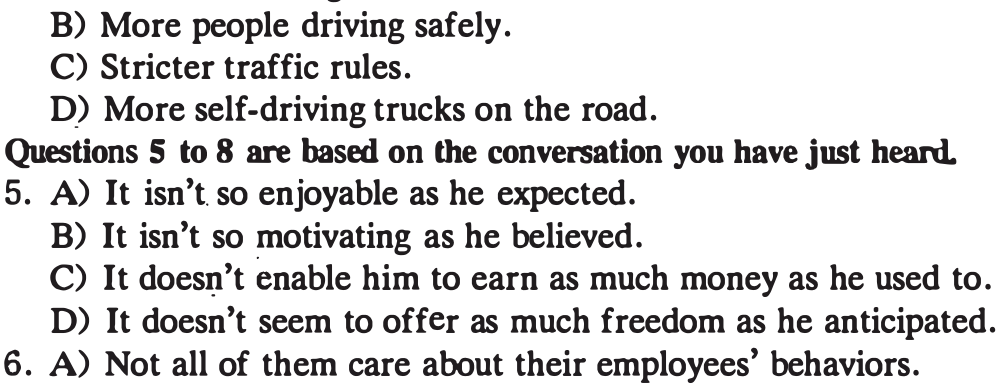
\includegraphics[width=\linewidth,height=.8\textheight,keepaspectratio]{2020-12-02.assets/char-001-line-014.png}\par

\begin{itemize}[leftmargin=2em,itemsep=.2em,topsep=.4em]\item[B.] More people driving safely.
\item[C.] Stricter traffic rules.
\item[D.] More self-driving trucks on the road.
\end{itemize}

5.


\begin{itemize}[leftmargin=2em,itemsep=.2em,topsep=.4em]\item[A.] It isn't so enjoyable as he expected.
\item[B.] It isn't so motivating as he believed.
\item[C.] It doesn't enable him to earn as much money as he used to.
\item[D.] It doesn't seem to offer as much freedom as he anticipated.
\end{itemize}

6.


\begin{itemize}[leftmargin=2em,itemsep=.2em,topsep=.4em]\item[A.] Not all of them care about their employees' behaviors.
\end{itemize}

\begin{itemize}[leftmargin=2em,itemsep=.2em,topsep=.4em]\item[B.] \textbf{Few of them are aware of their employees' feelings.}
\item[C.] \textbf{Few of them offer praise and reward to their employees.}
\item[D.] \textbf{Not all of them know how to motivate their employees.}
\end{itemize}

\noindent\begin{tabularx}{\linewidth}{@{}lXXXX@{}}\textbf{7.} & \textbf{A.} \textbf{Job satisfaction.} & \textbf{B.} \textbf{Self-awareness.} & \textbf{C.} \textbf{Autonomy.} & \textbf{D.} \textbf{Money.}\\\end{tabularx}\par

\textbf{8.}


\begin{itemize}[leftmargin=2em,itemsep=.2em,topsep=.4em]\item[A.] \textbf{The importance of cultivating close relationships with clients.}
\item[B.] \textbf{The need for getting recommendations from their managers.}
\item[C.] \textbf{The advantages of permanent full-time employment.}
\item[D.] \textbf{The way to explore employees' interests and talents.}
\end{itemize}

\subsection*{\textbf{Section B}}


\textbf{Directions: }\textbf{\textit{In this section, you will hear two JXlSsages. At the end of each passage, you will hear three or}} \textbf{\textit{four questions. Both the JXlSsage and the questions will be spoken only once. After you hear a question,}} \textbf{\textit{you must choose the best answer from the four choices marked A }}\textbf{) , }\textbf{\textit{B }}\textbf{) , C ) }\textbf{\textit{and D }}\textbf{) . }\textbf{\textit{Then mark}} \textbf{\textit{the corresponding letter on Answer Sheet 1 with a single li ne through the centre.}}


\textbf{Questions 9 to 11 are based on the passage you have just heard.}


\textbf{9.}


\begin{itemize}[leftmargin=2em,itemsep=.2em,topsep=.4em]\item[A.] \textbf{Consumers visualize their activities in different weather.}
\item[B.] \textbf{Good weather triggers consumers' desire to go shopping.}
\item[C.] \textbf{Weather conditions influence consumers' buying behavior.}
\item[D.] \textbf{Consumers' mental states change with the prices of goods.}
\end{itemize}

\noindent\begin{tabularx}{\linewidth}{@{}lXXXX@{}}\textbf{10.} & \textbf{A.} \textbf{Active consumption.} & \textbf{B.} \textbf{Direct correlation.} & \textbf{C.} \textbf{Individual association.} & \textbf{D.} \textbf{Mental visualization.}\\\end{tabularx}\par

\textbf{11.}


\begin{itemize}[leftmargin=2em,itemsep=.2em,topsep=.4em]\item[A.] \textbf{Enabling them to simplify their mathematical formulas.}
\item[B.] \textbf{Helping them determine what to sell and at what price.}
\item[C.] \textbf{Enabling them to sell their products at a higher price.}
\item[D.] \textbf{Helping them advertise a greater variety of products.}
\end{itemize}

\textbf{Questions 12 to 15 are based on the passage you have just heard.}


\textbf{12.}


\begin{itemize}[leftmargin=2em,itemsep=.2em,topsep=.4em]\item[A.] \textbf{A naturally ventilated office is more comfortable.}
\item[B.] \textbf{A cool office will boost employees' productivity.}
\item[C.] \textbf{Office air-conditioning should follow guidebooks.}
\item[D.] \textbf{Air-conditioning improves ventilation in the office.}
\end{itemize}

\textbf{13.}


\begin{itemize}[leftmargin=2em,itemsep=.2em,topsep=.4em]\item[A.] \textbf{People in their comfort zone of temperature are more satisfied with their productivity.}
\item[B.] \textbf{People in different countries vary in their tolerance to uncomfortable temperatures.}
\item[C.] \textbf{Twenty-two degrees is the optimal temperature for office workers.}
\item[D.] \textbf{There is a range of temperatures for people to feel comfortable.}
\end{itemize}

\textbf{14.}


\begin{itemize}[leftmargin=2em,itemsep=.2em,topsep=.4em]\item[A.] \textbf{It will have no negative impact on work.}
\item[B.] \textbf{It will be immediately noticeable.}
\item[C.] \textbf{It will sharply decrease work efficiency.}
\item[D.] \textbf{It will cause a lot of discomfort.}
\end{itemize}

\textbf{15.}


\begin{itemize}[leftmargin=2em,itemsep=.2em,topsep=.4em]\item[A.] \textbf{They tend to favor lower temperatures.}
\item[B.] \textbf{They suffer from rapid temperature changes.}
\item[C.] \textbf{They are not bothered by temperature extremes.}
\item[D.] \textbf{They become less sensitive to high temperatures.}
\end{itemize}

\subsection*{\textbf{Section C}}


\textbf{Directions: }\textbf{\textit{In this section, you will hear three recordings of lectures or talks followed by three or four}} \textbf{\textit{questions. The recordings will be played only once. After you hear a question }}, \textbf{\textit{you must choose the best}} \textbf{\textit{answer frcm the four choices marked A), B), }}\textbf{C) }\textbf{\textit{and }}\textbf{D). }\textbf{\textit{Then mark the corresponding letter on Answer}} \textbf{\textit{Sheet 1 with a single line through the centre.}}


\textbf{Questions 16 to 18 are based on the recording you have just heard.}


\textbf{16.}


\begin{itemize}[leftmargin=2em,itemsep=.2em,topsep=.4em]\item[A.] \textbf{It overlooked the possibility that emotions may be controlled.}
\item[B.] \textbf{It ignored the fact that emotions are personal and subjective.}
\item[C.] \textbf{It classified emotions simply as either positive or negative.}
\item[D.] \textbf{It measured positive and negative emotions independently.}
\end{itemize}

\textbf{17.}


\begin{itemize}[leftmargin=2em,itemsep=.2em,topsep=.4em]\item[A.] \textbf{Sitting alone without doing anything seemed really distressing.}
\item[B.] \textbf{Solitude adversely affected the participants' mental well-being.}
\item[C.] \textbf{Sitting alone for 15 minutes made the participants restless.}
\item[D.] \textbf{Solitude had a reductive effect on high-arousal emotions.}
\end{itemize}

\textbf{18.}


\begin{itemize}[leftmargin=2em,itemsep=.2em,topsep=.4em]\item[A.] \textbf{It proved hard to depict objectively.}
\item[B.] \textbf{lt went hand in hand with sadness.}
\item[C.] \textbf{It helped increase low-arousal emotions.}
\item[D.] \textbf{It tended to intensify negative emotions.}
\end{itemize}

\textbf{Questions 19 to 21 are based on the recording you have just heard.}


\textbf{19.}


\begin{itemize}[leftmargin=2em,itemsep=.2em,topsep=.4em]\item[A.] \textbf{It uses up much less energy than it does in deep thinking.}
\item[B.] It remains inactive without burning calories noticeably.
\item[C.] It continues to burn up calories to help us stay in shape.
\item[D.] \textbf{It consumes almost a quarter of the body's total energy.}
\end{itemize}

\textbf{20.}


\begin{itemize}[leftmargin=2em,itemsep=.2em,topsep=.4em]\item[A.] \textbf{Much of the consumption has nothing to do with conscious activities.}
\item[B.] \textbf{It has something to do with the difficulty of the activities in question.}
\item[C.] \textbf{Energy usage devoted to active learning accounts for a big part of it.}
\item[D.] \textbf{A significant amount of it is for performing difficult cognitive tasks.}
\end{itemize}

\textbf{21.}


\begin{itemize}[leftmargin=2em,itemsep=.2em,topsep=.4em]\item[A.] \textbf{It is believed to remain basically constant.}
\item[B.] \textbf{It is a prerequisite for any mental activity.}
\item[C.] \textbf{It is conducive to relieving mental exhaustion.}
\item[D.] \textbf{It is thought to be related to food consumption.}
\end{itemize}

\textbf{Questions 22 to 25 are based on the reconling you have just heard.}


\textbf{22.}


\begin{itemize}[leftmargin=2em,itemsep=.2em,topsep=.4em]\item[A.] \textbf{Job candidates rarely take it seriously.}
\item[B.] \textbf{Job seekers tend to have a ready answer.}
\item[C.] \textbf{Job seekers often feel at a loss where to start in answering it.}
\item[D.] \textbf{Job candidates can respond freely due to its open-ended nature.}
\end{itemize}

\textbf{23.}


\begin{itemize}[leftmargin=2em,itemsep=.2em,topsep=.4em]\item[A.] \textbf{Follow their career coaches' guidelines.}
\item[B.] \textbf{Strive to take control of their narrative.}
\item[C.] \textbf{Do their best to impress the interviewer.}
\item[D.] \textbf{Repeat the information on their resume.}
\end{itemize}

\textbf{24.}


\begin{itemize}[leftmargin=2em,itemsep=.2em,topsep=.4em]\item[A.] \textbf{To reflect on their past achievements as well as failures.}
\item[B.] \textbf{To produce examples for different interview questions.}
\item[C.] \textbf{To discuss important details they are going to present.}
\item[D.] \textbf{To identify a broad general strength to elaborate on.}
\end{itemize}

\textbf{25.}


\begin{itemize}[leftmargin=2em,itemsep=.2em,topsep=.4em]\item[A.] \textbf{Getting acquainted with the human resources personnel.}
\item[B.] \textbf{Finding out why the company provides the job opening.}
\item[C.] \textbf{Figuring out what benefits the company is able to offer them.}
\item[D.] \textbf{Tailoring their expectations to the company's long-term goal.}
\end{itemize}

\noindent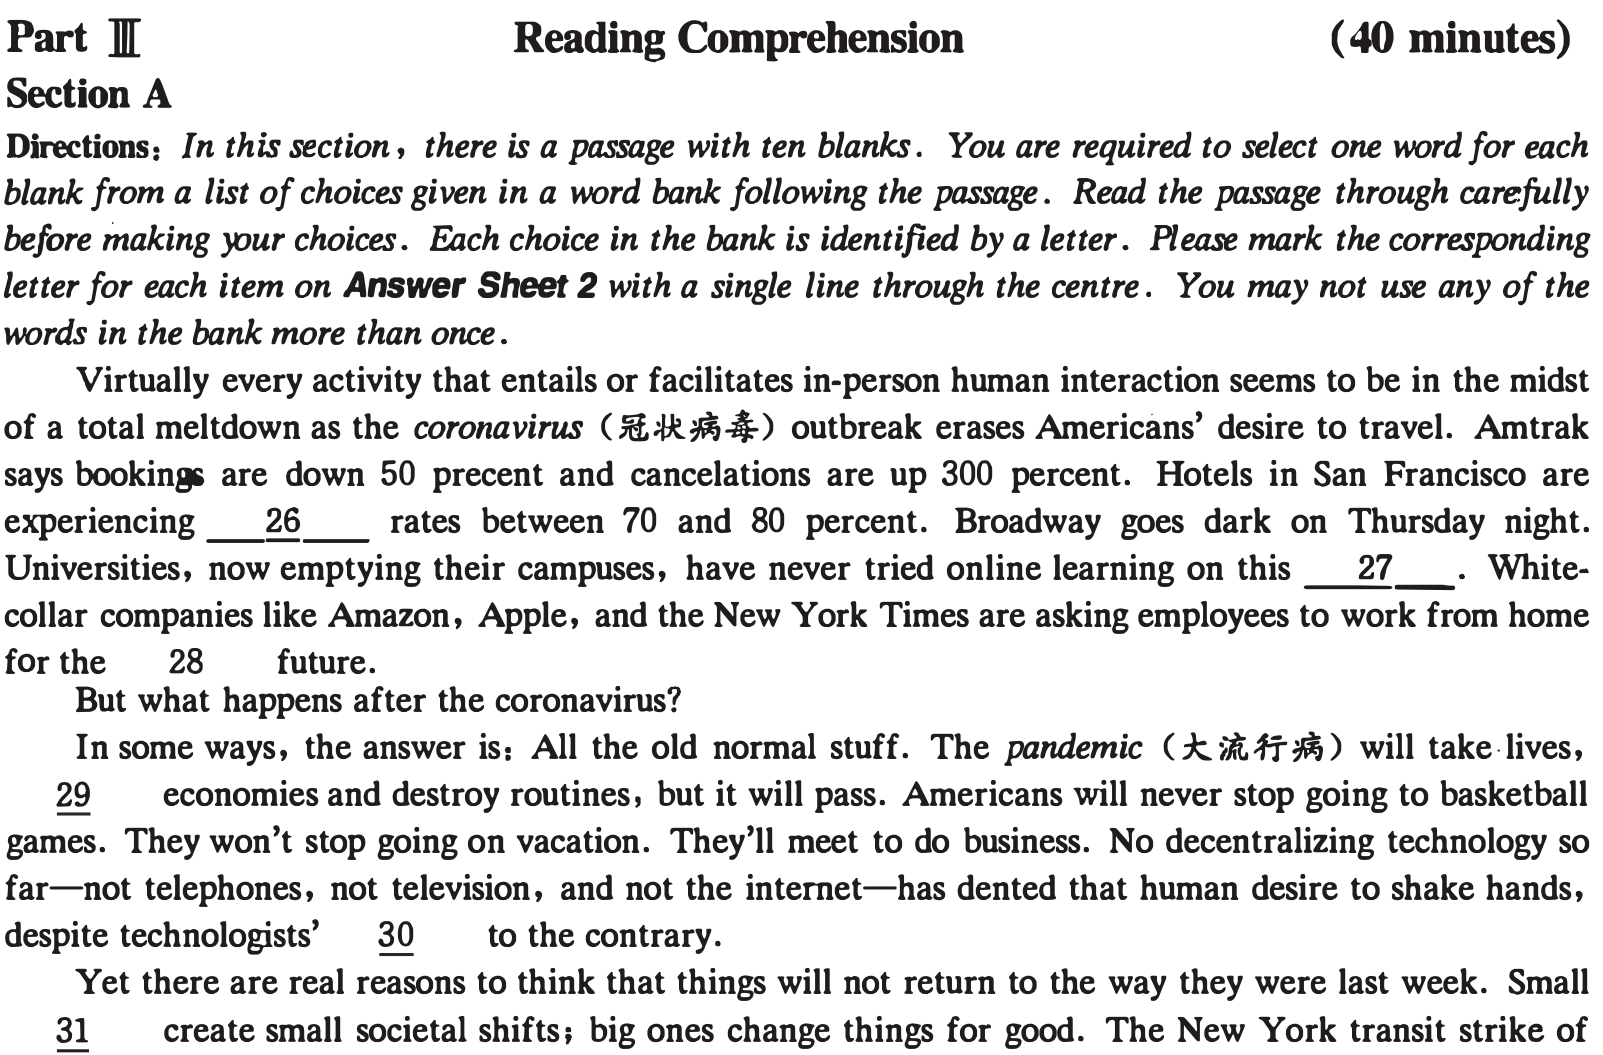
\includegraphics[width=\linewidth,height=.8\textheight,keepaspectratio]{2020-12-02.assets/char-003-line-013.png}\par

\noindent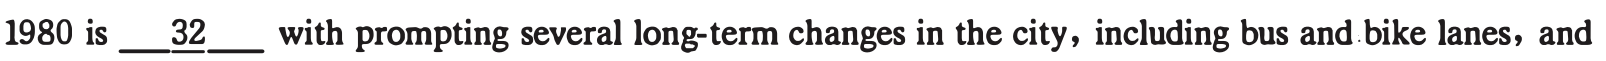
\includegraphics[width=\linewidth,height=.8\textheight,keepaspectratio]{2020-12-02.assets/char-004-line-000.png}\par

\begin{itemize}[leftmargin=2em,itemsep=.2em,topsep=.4em]\item[A.] \textbf{credentials}
\item[B.] \textbf{credited}
\item[C.] \textbf{cumulative}
\item[D.] \textbf{disruptions}
\item[E.] \textbf{federal}
\item[F.] \textbf{foreseeable}
\item[G.] \textbf{predictions}
\item[H.] \textbf{preference}
\item[I.] \textbf{scale}
\item[J.] \textbf{strangle} \textbf{0) wedge}
\item[K.] \textbf{subtle}
\item[L.] \textbf{summoned •}
\item[M.] \textbf{survive}
\item[N.] \textbf{vacancy}
\end{itemize}

\subsection*{\textbf{Section B}}


\textbf{Directions: }\textbf{\textit{In this section, you are going to read a passage with ten statements attached to it. F.ach}} \textbf{\textit{statement contains information given in one of the paragraphs. Identify the paragraph from which the}} \textbf{\textit{information is derived. You may choose a paragraph more than once. F.ach paragraph is marked with a}} \textbf{\textit{letter. Answer the questions by marking the corresponding letter on Answer Sheet 2.}}


\noindent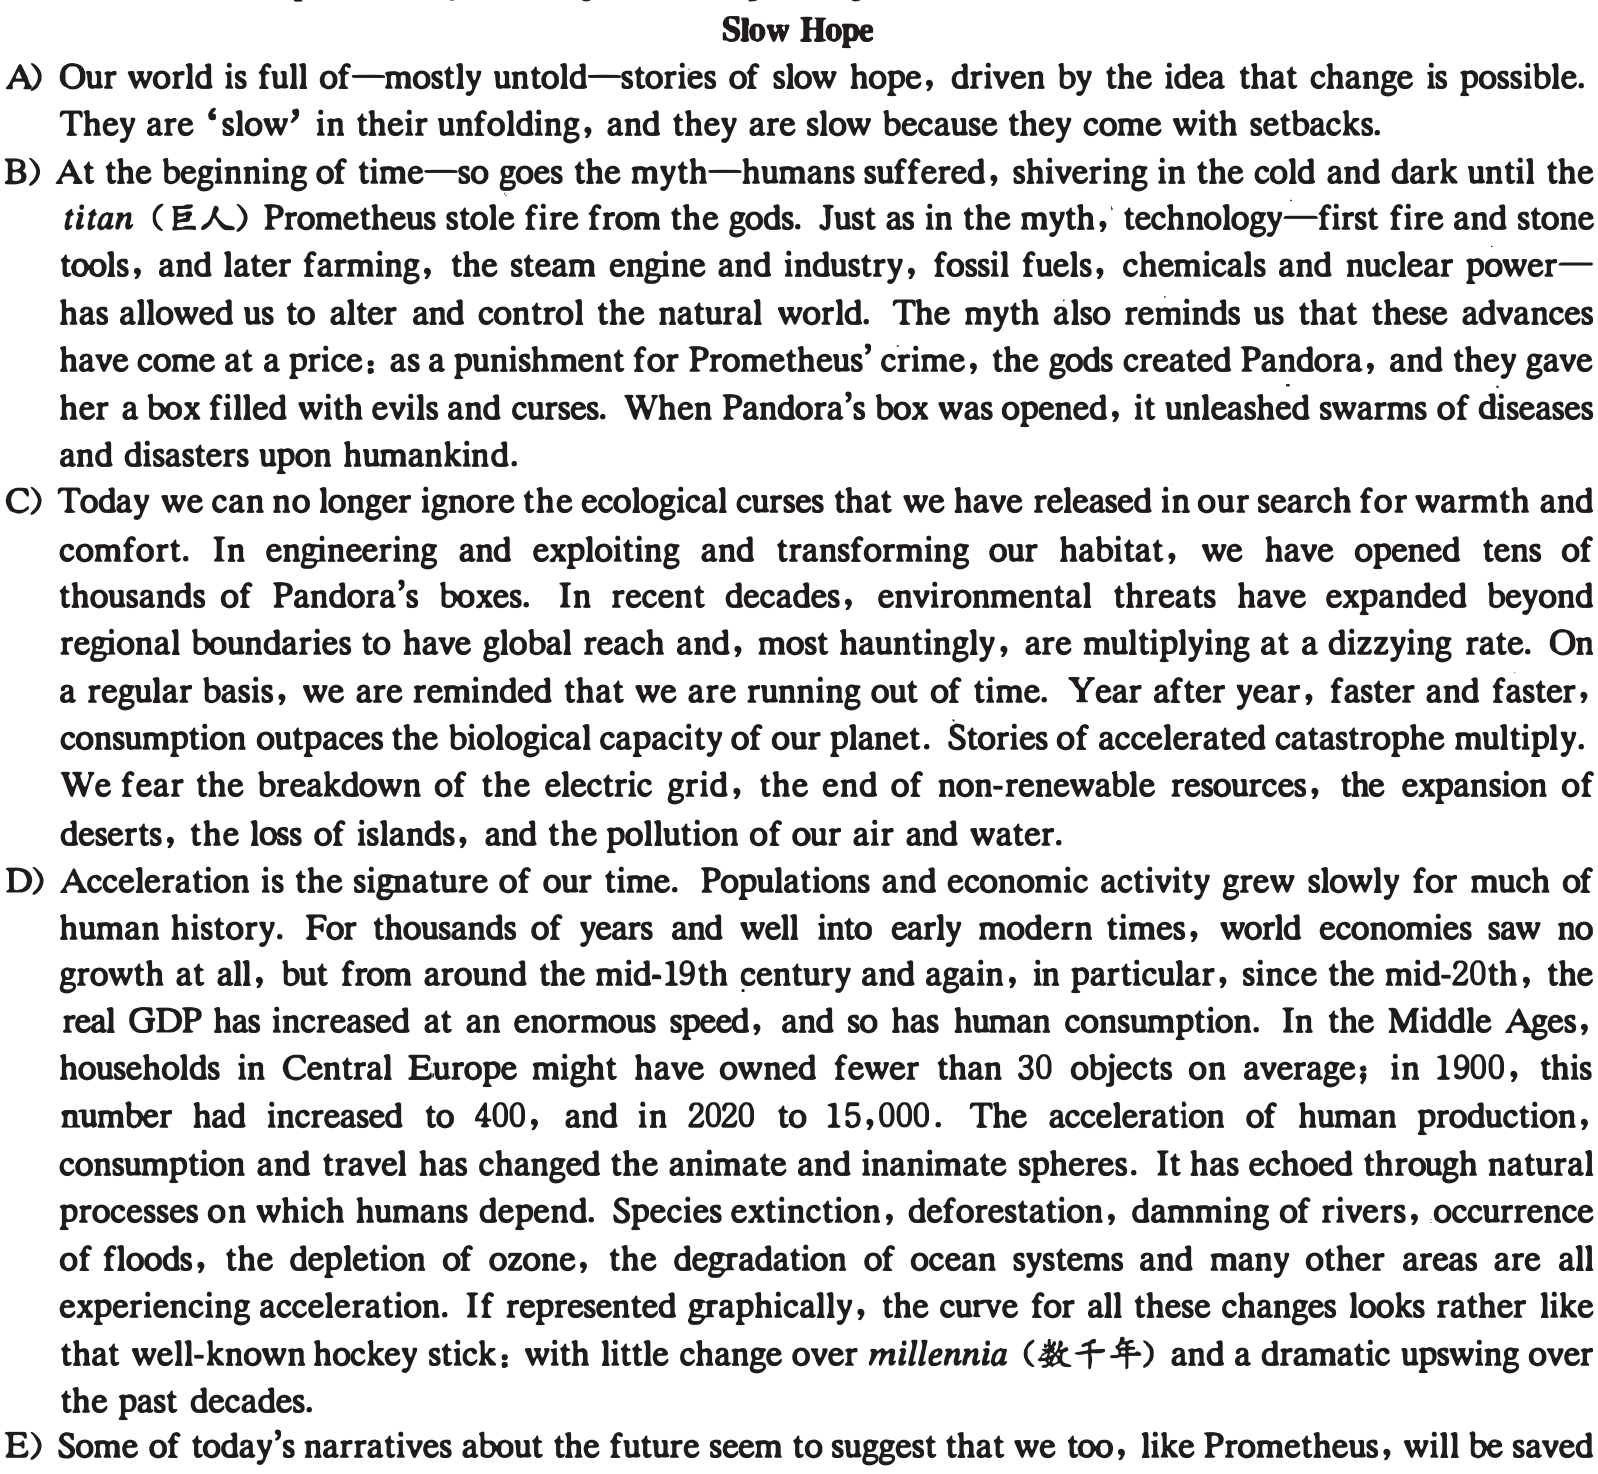
\includegraphics[width=\linewidth,height=.8\textheight,keepaspectratio]{2020-12-02.assets/char-004-line-004.png}\par

\textbf{by a new Hercules, a divine engineer, someone who will mastermind, manoeuvre and manipulate our} \textbf{planet. They suggest that geoengineering, cold fusion or faster-than-light spaceships might transcend} \textbf{once and for all the terrestrial constraints of rising temperatures, lack of energy, scarcity of food, lack} \textbf{of space, mountains of waste, polluted water-you name it.}


F) \textbf{Yet, if we envisage our salvation to come from a }\textbf{\textit{deus ex machina }}\textbf{(W\#-i!l.:t..\#), from a divine engineer} \textbf{or a tech solutionist who will miraculously conjure up a new source of energy or another cure-all with} \textbf{revolutionary potency, we might be looking in the wrong place. The fact that we now imagine our} \textbf{planet as a whole does not mean that the 'rescue' of our planet will come with one big global stroke of} \textbf{genius and technology. It will more likely come by many small acts. Global heating and environmental} \textbf{degradation are not technological problems. They are highly political issues that are informed by} \textbf{powerful interests. Moreover, if history is a guide, then we can assume that any major transformations} \textbf{will once again be followed by a huge set of unintended consequences. So what do we do?}


G) \textbf{This much is clear: we need to find ways that help us flatten the hockey-stick curves that reflect our} \textbf{ever-faster pace of ecological destruction and social acceleration. If we acknowledge that human} \textbf{manipulation of the Earth has been a\textperiodcentered{} destructive force, we can also imagine that human endeavours} \textbf{can help us build a less destructive world in the centuries to come. We might keep making mistakes.} \textbf{But we will also keep learning from our mistakes.}


H) \textbf{To counter the fears of disaster, we need to identify stories, visions and actions that work quietly}


\noindent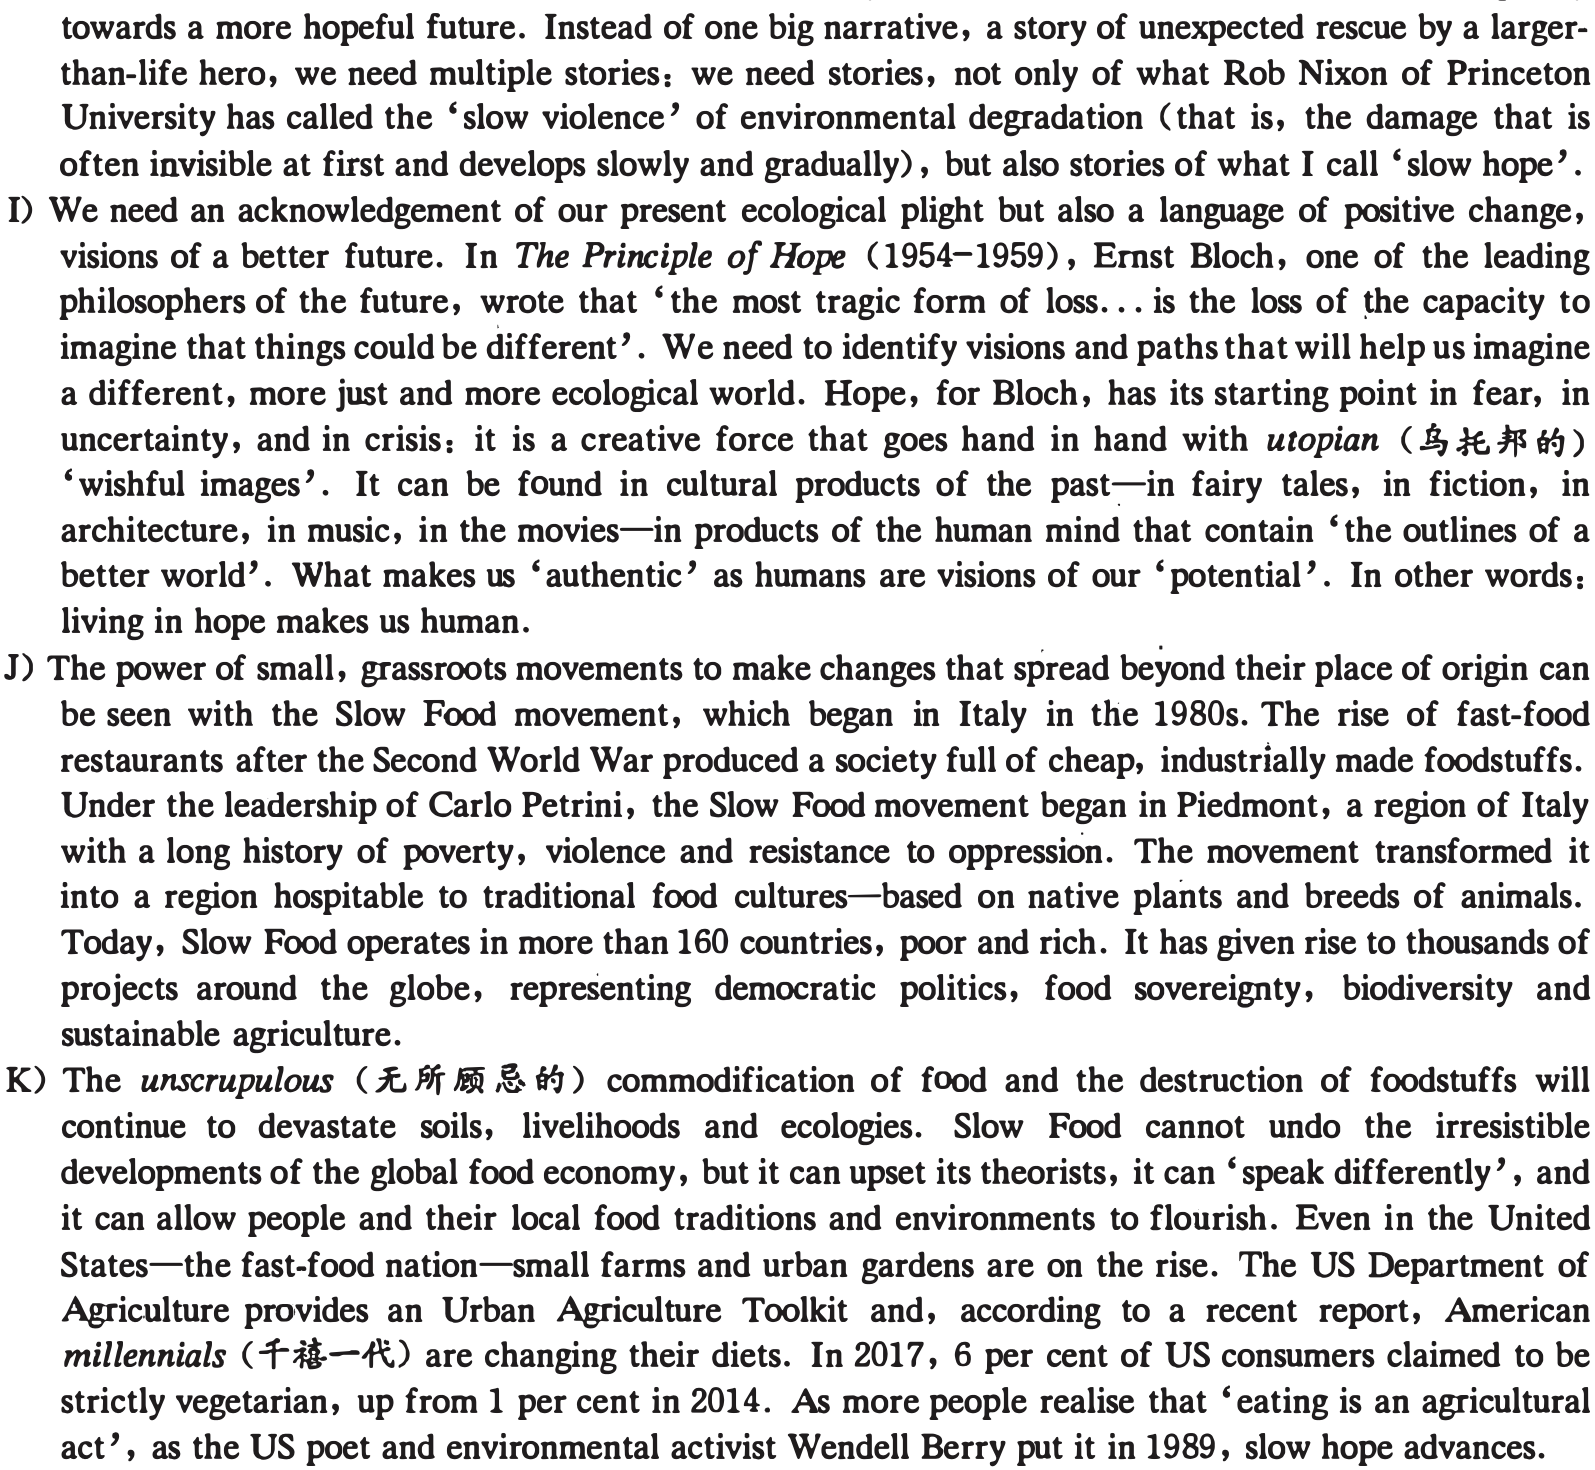
\includegraphics[width=\linewidth,height=.8\textheight,keepaspectratio]{2020-12-02.assets/char-005-line-004.png}\par

\textbf{36. It seems some people today dream that a cutting-edge new technology might save them from the}


\textbf{present ecological disaster.}


\textbf{37. According to one great thinker, it is most unfortunate if we lose the ability to think differently.}


\textbf{38. Urgent attention should be paid to the ecological problems we have created in our pursuit of a}


\textbf{comfortable life.}


\textbf{39. Even in the fast-food nation America, the number of vegetarians is on the rise.}


\textbf{40. The deterioration of the ecological system is accelerating because of the dramatic increase of human}


\textbf{production and consumption.}


\textbf{41. It is obvious that solutions must be found to curb the fast worsening environment and social}


\textbf{acceleration.}


\textbf{42. Many people believe changing the world is possible, though it may take time and involve setbacks.}


\textbf{43. It might be wrong to expect that our world would be saved at one stroke with some miraculous}


\textbf{technology.}


\textbf{44. It is human nature to cherish hopes for a better world.}


\textbf{45. Technology has given us humans the power to change the natural world, but we have paid a price for}


\textbf{the change.}


\subsection*{\textbf{Section C}}


\textbf{Directions: }\textbf{\textit{There are 2 JXlSsages in this section. Each pcmage is followed by sane questions or unfinished}} \textbf{\textit{statements. For each of them there are four choices marked }}\textbf{A), B), C) }\textbf{\textit{and }}\textbf{D). }\textbf{\textit{You should decide on the}} \textbf{\textit{best choice and mark the corresponding letter on Answer Sheet 2 with a single line through the centre.}}


\subsection*{\textbf{Passage One}}


\textbf{Questions 46 to 50 are based on the following passage.}


\noindent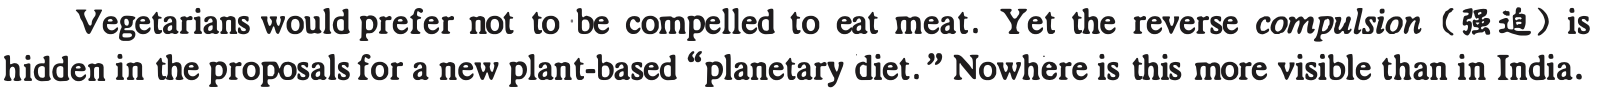
\includegraphics[width=\linewidth,height=.8\textheight,keepaspectratio]{2020-12-02.assets/char-006-line-020.png}\par

\textbf{Earlier this year, the EAT-Lancet Commission released its global report on nutrition and called for a} \textbf{global shift to a more plant-based diet and for "substantially reducing consumption of animal source} \textbf{foods." In countries like India, that call could become a tool to aggravate an already tense political} \textbf{situation and stress already undernourished populations.}


\noindent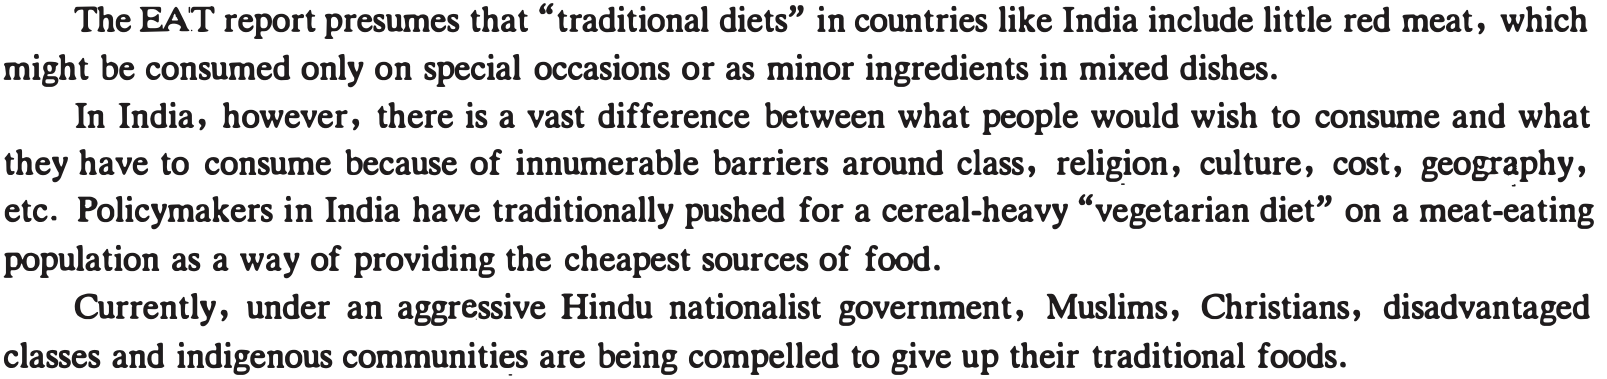
\includegraphics[width=\linewidth,height=.8\textheight,keepaspectratio]{2020-12-02.assets/char-006-line-022.png}\par

\textbf{. . None of these concerns seem to have been appreciated by the EAT-Lancet Commissicm's} \textbf{representative, Brent Loken, who said "India has got such a great example" in sourcing protein from} \textbf{plants.}


\textbf{But how much of a model for the world is India's vegetarianism? In the Global Hunger Index 2019,} \textbf{the country ranks 102nd out of 117. Data from the National Family Health Survey indicate that only 10} \textbf{percent of infants of 6 to 23 months are adequately fed.}


\textbf{Which is why calls for a plant-based diet modeled on India risk offering another whip with which to} \textbf{beat already vulnerable communities in developing countries.}


\textbf{A diet directed at the affluent West fails to recognize that in low-income countries undernourished} \textbf{children are known to benefit from the consumption of milk and other animal source foods, improving} \textbf{cognitive functions, while reducing the prevalence of nutritional deficiencies as well as mortality.}


\textbf{•} \textbf{EAT-Lancet claimed its intention was to "spark conversations" among all Indian stakeholders. Yet} \textbf{vocal critics of the food processing industry and food fortification strategies have been left out of the} \textbf{debate; But the most conspicuous omission may well be the absence of India's farmers.}


\textbf{The government, however, seems to have given the report a thumbs-up. Rather than addressing} \textbf{chronic hunger and malnutrition through an improved access to wholesome and nutrient-dense foods, the} \textbf{government is opening the door for company-dependent solutions, ignoring the environmental and} \textbf{economic cost, which will destroy local food systems. It's a model full of danger for future generations.}


\textbf{46. What is more visible in India than anywhere else according to the passage?}


\begin{itemize}[leftmargin=2em,itemsep=.2em,topsep=.4em]\item[A.] \textbf{People's positive views on the proposals for a "planetary diet."}
\item[B.] \textbf{People's reluctance to be compelled to eat plant-based food.}
\item[C.] \textbf{People's preferences for the kind of food they consume.}
\item[D.] \textbf{People's unwillingness to give up their eating habits.}
\end{itemize}

\textbf{47. What would the EAT-Lancet Commission's report do to many people in countries like India?}


\begin{itemize}[leftmargin=2em,itemsep=.2em,topsep=.4em]\item[A.] \textbf{Radically change their dietary habits.}
\item[B.] \textbf{Keep them further away from politics.}
\item[C.] \textbf{Make them even more undernourished.}
\item[D.] \textbf{Substantially reduce their food choices.}
\end{itemize}

\textbf{48. What do we learn from the passage about food consumption in India?}


\begin{itemize}[leftmargin=2em,itemsep=.2em,topsep=.4em]\item[A.] \textbf{People's diet will not change due to the EAT-Lancet report.}
\item[B.] \textbf{Many people simply do not have access to foods they prefer.}
\item[C.] \textbf{There is a growing popularity of a cereal-heavy vegetarian diet.}
\item[D.] \textbf{Policymakers help remove the barriers to people's choice of food.}
\end{itemize}

\textbf{49. What does the passage say about a plant-based diet modeled on India?}


\begin{itemize}[leftmargin=2em,itemsep=.2em,topsep=.4em]\item[A.] \textbf{It may benefit populations whose traditional diet is meat-based.}
\item[B.] \textbf{It may be .another blow to the economy in developing countries.}
\item[C.] \textbf{It may help narrow the gap between the rich and poor countries.}
\item[D.] \textbf{It may worsen the nourishment problem in low-income countries.}
\end{itemize}

\textbf{50. How does the Indian government respond to the EAT-Lancet Commission's proposals?}


\begin{itemize}[leftmargin=2em,itemsep=.2em,topsep=.4em]\item[A.] \textbf{It accepts them at the expense of the long-term interests of its people.}
\item[B.] \textbf{It intends them to spark.conversations among all Indian stakeholders.}
\item[C.] \textbf{It gives them approval regardless of opposition from nutrition experts.}
\item[D.] \textbf{It welcomes them as a tool to address chronic hunger and malnutrition.}
\end{itemize}

\noindent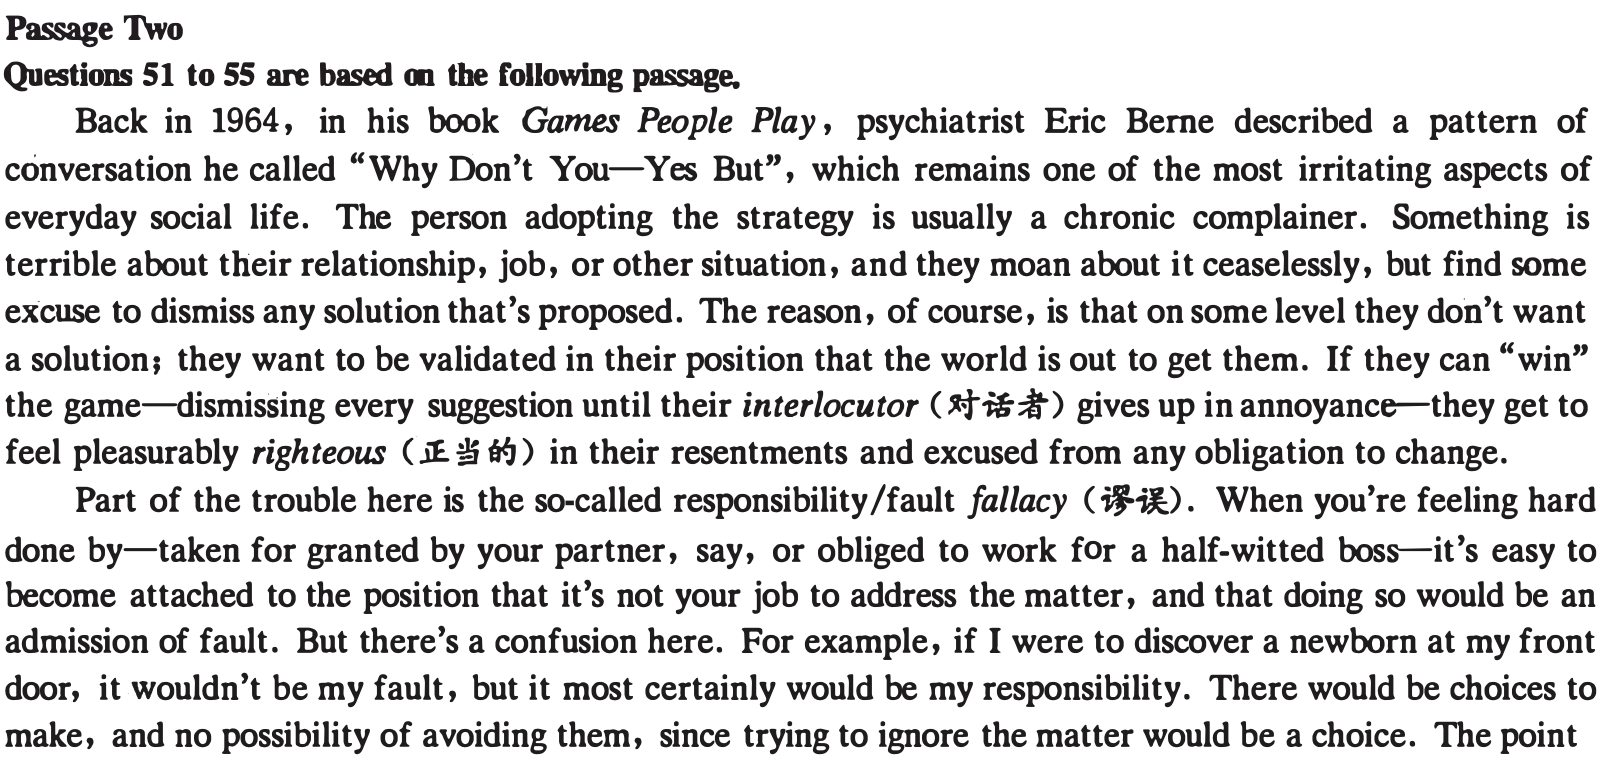
\includegraphics[width=\linewidth,height=.8\textheight,keepaspectratio]{2020-12-02.assets/char-007-line-012.png}\par

\textbf{is that what goes for the baby on the doorstep is true in all casess even if the other person is 100\% in the wrong,} \textbf{there’s nothing to be gained, long-term, from using this as a justification to evade responsibility.}


\textbf{Should you find yourself on the receiving end of this kind of complaining, there’s an ingenious way to shut it down} \textbf{—which is to agree with it, ardently. Psychotherapist Lori Gottlieb describes this as “over validation”. For} \textbf{one thing, you’ll be spared further moaning, since the other person’s motivation was to confirm her beliefs, and} \textbf{now you’re confirming them. But for another, as Gottlieb notes, people confronted with over-validation often hear} \textbf{their complaints afresh and start arguing back. The notion that they’re utterly powerless suddenly seems} \textbf{unrealistic—not to mention rather annoying—so they’re prompted instead to generate ideas about how they} \textbf{might change things.}


\textbf{“And then, sometimes, something magical might happen,” Gottlieb writes. The other person “might realise she’s} \textbf{not as trapped as you are saying she is, or as she feels.” Which illustrates the irony of the responsibility} \textbf{fault fallacy: evading responsibility feels comfortable, but turns out to be a prison; whereas assuming} \textbf{responsibility feels unpleasant, but ends up being freeing.}


\textbf{51. What is characteristic of a chronic complainer, according to psychiatrist Eric Berne?}


\begin{itemize}[leftmargin=2em,itemsep=.2em,topsep=.4em]\item[A.] \textbf{They only feel angry about their ill treatment and resent whoever tries to help.}
\item[B.] \textbf{They are chronically unhappy and ceaselessly find fault with people around them.}
\item[C.] \textbf{They constantly dismiss others’ proposals while taking no responsibility for tackling the problem.}
\item[D.] \textbf{They lack the kn w e g a d basic skills required for successful conversations with their interlocutors.}
\end{itemize}

\textbf{52. What does the author try to illustrate with the example of the newborn on one’s doorstep?}


\begin{itemize}[leftmargin=2em,itemsep=.2em,topsep=.4em]\item[A.] \textbf{People tend to think that one should not be held responsible for others’ mistakes.}
\item[B.] \textbf{It is easy to become attached to the position of overlooking one’s own fault.}
\item[C.] \textbf{People are often at a loss when confronted with a number of choices.}
\item[D.] \textbf{A distinction should be drawn between responsibility and fault.}
\end{itemize}

\textbf{53. What does the author advise people to do to chronic complainers?}


\begin{itemize}[leftmargin=2em,itemsep=.2em,topsep=.4em]\item[A.] \textbf{Stop them from going further by agreeing with them.}
\item[B.] \textbf{Listen to their complaints ardently and sympathetically.}
\item[C.] \textbf{Ask them to validate their beliefs with further evidence.}
\item[D.] \textbf{Persuade them to clarify the confusion they have caused.}
\end{itemize}

\textbf{54. What happens when chronic complainers receive over-validation?}


\begin{itemize}[leftmargin=2em,itemsep=.2em,topsep=.4em]\item[A.] \textbf{They are motivated to find ingenious ways to persuade their interlocutor.}
\item[B.] \textbf{They are prompted to come up with ideas for making possible changes.}
\item[C.] \textbf{They are stimulated to make more complaints.}
\item[D.] \textbf{They are encouraged to start arguing back.}
\end{itemize}

\textbf{55. How can one stop being a chronic complainer according to the author?}


\begin{itemize}[leftmargin=2em,itemsep=.2em,topsep=.4em]\item[A.] \textbf{Analysing the so-called responsibility/fault fallacy.}
\item[B.] \textbf{Avoiding hazardous traps in everyday social life.}
\item[C.] \textbf{Assuming responsibility to free oneself.}
\item[D.] \textbf{Awaiting something magical to happen.}
\end{itemize}

\subsection*{\textbf{Part IV} \textbf{Translation} \textbf{(30 minutes)}}


\textbf{Directions: For this part, you are allowed 30 minutes to translate a passage from Chinese into English. You should write} \textbf{your answer on Answer Sheet 2.}


\CJKunderline{港珠澳大桥(}Hong Kong-Zhuhai-Macau Bridge)全长55公里,是我国一项不同寻常的工程壮举。大桥将三个城市连接起来,是世界上最长的跨海桥梁和隧道系统。大桥将三个城市之间的旅行时间从3小时缩短到30分钟。这座跨度巨大的钢筋混凝土大桥充分证明中国有能力建造创纪录的巨型建筑。它将助推区域一体化,促进经济增长。大桥是中国发展自己的大湾区总体规划的关键。中国希望将大湾区建成在技术创新和经济繁荣上能与旧金山、纽约和东京的湾区相媲美的地区。

\end{document}